\chapter{Results and Discussion}
Up to this point, we have laid the theoretical and methodological foundations of our investigation:  
from the gravitational wave theory, to the astrophysical context of white dwarfs and their host galaxies, the principles of gravitational wave detection, and finally the construction of the simulated populations used in this work.  
In this chapter, we finally turn to the quantitative results on the generation of the corresponding gravitational wave signal.  
We begin by applying the computational pipeline described in the previous chapter to our final galaxy catalog, extracting the gravitational wave signal from the simulated populations of binary white dwarfs.  
The resulting spectra are then compared to the LISA sensitivity curve to verify the detectability of an extragalactic background.  
We then discuss the frequency distribution and amplitude characteristics of the simulated signals, as well as the physical reasons underlying our results, and their implications for future space-based gravitational wave detectors.

\section{The Signal Computation}
In order to compute the total extragalactic DWDs gravitational background, we must apply an iterative process to each galaxy in the final catalog, which consists of the following steps:
\begin{itemize}
    \item Compute the right $N_{astro}$ using the~\eqref{eq: scale by mass}
    \item Scale the fixed population accordingly with a sampling with replacement method, creating the full-size galaxy simulation.
    \vspace{1.5mm}\\
    At this point for each binary system in this astrophysical population we:
    \begin{itemize}
        \item Compute the gravitational wave signal using~\eqref{eq: the strain we use}\footnote{Note here that all the binaries within the same galaxy are given the same distance from us. This approximation is considered t be valid since the distance of the galaxy is much much bigger the its size, and thus the maximum possible distance between two binaries within the same galaxy.} and the corresponding $PSD$ using~\eqref{eq: ASD definition} and~\eqref{eq: PSD definition};
        \item Sum the total PSD of the binaries whose frequencies fall within the same LISA's frequency bin, using~\eqref{eq: total PSD};
        \item Plot the total binned signals on LISA's curve.
    \end{itemize}
\end{itemize}
\subsubsection{LISA's sensitivity curve}
The LISA curve is constantly updated when new gravitational wave components that can affect it are found, meaning that there are many different versions around.
The one we chose to use is the widely used version made by~\cite{Robson_2019}, which is written as:
\begin{equation}
    S_n = \frac{10}{3L^2} \left( P_{OMS}(f) + \frac{4P_{acc}(f)}{(2\pi f)^4} \right)\left( 1 + \frac{6}{10}\left(\frac{f}{f_*}\right)^2 \right) + S_c(f),
    \label{eq: LISA sensitivity curve by Robson}
\end{equation}
where $L=2.5 Gm$ is the LISA arm length, $f_*=19.09mHz$ and $P_{OMS}(f)$, $P_{acc}(f)$ and $S_c(f)$ are the expressions for the single-link optical metrology noise, the single test mass acceleration noise and the total Michaelson-style LISA data channel. 
The equations for these factors, as well as more detail on the curve that we chose, can be found in the article.
Doing this, the spectral distribution of the final resulting signal is plotted over the LISA's sensitivity curve\footnote{This particular curve is presented in~\cite{Robson_2019}.} in \textbf{Figure~\ref{fig: Final results plot}}
\begin{figure}[hb!]
    \begin{center}
        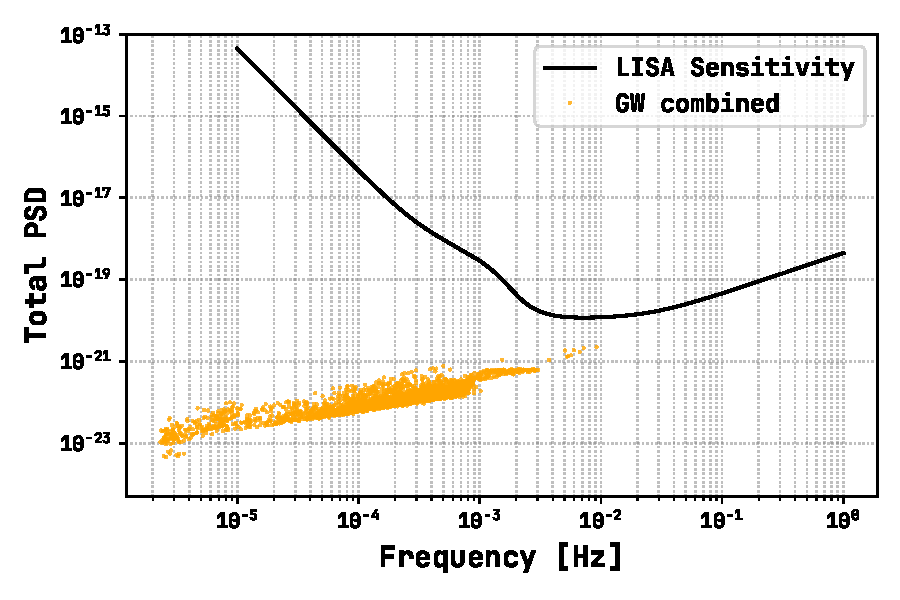
\includegraphics[width=0.8\textwidth]{images/Final_results_plot.pdf}
    \end{center}
    \caption{Total gravitational wave signal of the simulated Double White Dwarfs (DWDs) hosted by the $66,568$ galaxies of the final catalog, binned in $\sim 8\times10^{-9}Hz$ large frequency bins, representing LISA's spectral resoution. 
    Every orange dot represents the signal of a frequency bin, calculated by summing the Power Spectral Density (PSD) of every galaxy that it contained, using~\eqref{eq: total PSD}. 
    The dots are plotted on LISA's sensitivity curve, as found in~\cite{Robson_2019}, and appear to be about one order of magnitude below the minimum threshold of this curve.
    This results suggest that we should not expect LISA to be able to detect the unresolved extragalactic DWDs confusion foreground, at least under the assumptions and approximations adopted in this work.}\label{fig: Final results plot}
\end{figure}
Every orange dot in \textbf{Figure~\ref{fig: Final results plot}} represents a frequency bin, whose width is given by~\eqref{eq: LISA frequency resolution}, where the signal of a certain number of simulated binaries has been summed using~\eqref{eq: total PSD}.
As we can see, the resulting signal appears to be about one order of magnitude smaller than the minimum detectable strain for LISA across the whole band.  
This indicates that the stochastic contribution from extragalactic DWDs will not have a measurable impact on LISA’s sensitivity curve, at least under the assumptions of our population model and scaling relations.

\paragraph{Distribution of the sources.}
The simulated extragalactic binaries populate primarily the low-frequency range ($f \lesssim 2\,\mathrm{mHz}$), with the number of systems decreasing steeply at higher frequencies. 
Because of the nature of binary formation, at higher frequencies the binary system have had enough time to evolve, and have thus a broader range of orbital frequencies where to spread. 
Once they get high enough in the spectrum, the faster orbital decay of short-period binaries causes the absence of gravitational wave signals at higher frequencies.
% This means that, at higher frequencies, it is more likely for single binaries to occupy different bins.
Moreover, the spectral shape of the resulting background is positioned at frequencies that are similar to the expected Galactic foreground ones (corresponding to the slight bump at the left of the lowest point in the graph - this is better shown in \textbf{Figure~\ref{fig: LISA sens curve with noises}}), but with a significantly lower amplitude due to the much larger average distances.
Indeed, as shown in~\eqref{eq: the strain we use}, the gravitational wave amplitude scales inversely with the distance from the source, so even relatively nearby galaxies contribute far less per binary than the Milky Way population. 
The total number of galaxies in the local Universe, even if large, is not sufficient to compensate for this distance-induced amplitude suppression in the LISA band.
